%%!TEX encoding = UTF-8 Unicode 
\documentclass[oneside,a4paper]{report}

% Use utf-8 encoding for foreign characters
\usepackage[utf8]{inputenc}

% Setup for fullpage use
\usepackage{fullpage}
\usepackage[usenames,dvipsnames]{color}
%\usepackage{subfigure}
% \usepackage{boxedminipage}
\usepackage{listings}
\usepackage{booktabs}
\usepackage{setspace}

\linespread{1.6}

\lstdefinelanguage[ARM]{Assembler}%
  {morekeywords=[1]{.text,.globl,.align},%
  morekeywords=[2]{add,beq,bge,blt,bne,cmp,ldr,mov,mul,pop,push,%
    subs,vadd,vld1,vldm,vmov,vmul,vpadd,vpop,vpush},%
   morekeywords=[3]{f32,s32,i32},%
   keywordsprefix=.,%
   sensitive,%
   morecomment=[l]//,% nonstandard
   moredelim=*[directive]\#,%
   moredirectives={define,elif,else,endif,error,if,ifdef,ifndef,line,%
      include,pragma,undef,warning}%
  }[keywords,comments,directives]

\lstdefinelanguage{AssemblerC}%
  {morekeywords=[1]{},%
  morekeywords=[2]{while,return},%
   morekeywords=[3]{float,int32_t},%
   % keywordsprefix=.,%
   sensitive,%
   morecomment=[l]//,% nonstandard
   moredelim=*[directive]\#,%
   moredirectives={define,elif,else,endif,error,if,ifdef,ifndef,line,%
      include,pragma,undef,warning}%
  }[keywords,comments,directives]

\lstset{
  numbers=left,
  numberstyle=\tiny,
  numbersep=10pt,
  basicstyle=\small\ttfamily,
  keywordstyle=[1]\color{RedOrange},
  keywordstyle=[2]\color{RoyalBlue},
  keywordstyle=[3]\color{Mulberry},
  identifierstyle=,
  commentstyle=\color{OliveGreen},
  stringstyle=\ttfamily,
  directivestyle=\color{OliveGreen},
  showstringspaces=false
}

% This is now the recommended way for checking for PDFLaTeX:
\usepackage{ifpdf}

%\newif\ifpdf
%\ifx\pdfoutput\undefined
%\pdffalse % we are not running PDFLaTeX
%\else
%\pdfoutput=1 % we are running PDFLaTeX
%\pdftrue
%\fi

\ifpdf
\usepackage[pdftex]{graphicx}
\else
\usepackage{graphicx}
\fi

\usepackage[colorlinks=true,citecolor=OrangeRed,urlcolor=NavyBlue,linkcolor=ForestGreen]{hyperref}
\usepackage[all]{hypcap}

\title{ \textbf{ARM Cortex-A8} \\ \large{4810-1164 Modern Computer Architectures and System Software}}
\author{ \textbf{Daniel Heffernan} \\ Creative Informatics (M1) -- 48-116625 }

\begin{document}

\ifpdf
\DeclareGraphicsExtensions{.pdf, .jpg, .tif}
\else
\DeclareGraphicsExtensions{.eps, .jpg}
\fi

\maketitle

\chapter{Introduction}

It is very popular recently, and its popularity is marked by its use by Apple as the CPU in the Apple A4 SoC (System on Chip), which powers Apple's iPad and iPhone 4. It is also notable for being the first implementation of the ARMv7 instruction set architecture which includes NEON \cite{Gris}, the \emph{single instruction, multiple data} (SIMD) unit which implements floating point (VFPv3) and SIMD (Advanced SIMD) instruction sets, and for operating at speeds of up to 1GHz in very low-power environments (sub-1W, and often around 300mW) \cite{Williamson}.

There are three Cortex series: Cortex-A, Cortex-R and Cortex-M. They are so named because of each series' ARMv7 instruction set profile. ARMv7-A is one of three available profiles of ARMv7 \cite[p. A1-4]{ARMRef}, and is used in the Cortex-A series. Cortex-R uses ARMv7-R, which is a real-time variant which uses a \emph{Protected Memory System Architecture} (PMSA) instead of ARMv7-A's \emph{Virtual Memory System Architecture} (VMSA). The Cortex-M series processors use the ARMv7-M profile, which is a microcontroller variant of ARMv7.

\begin{figure}[htbp]
	\centering
	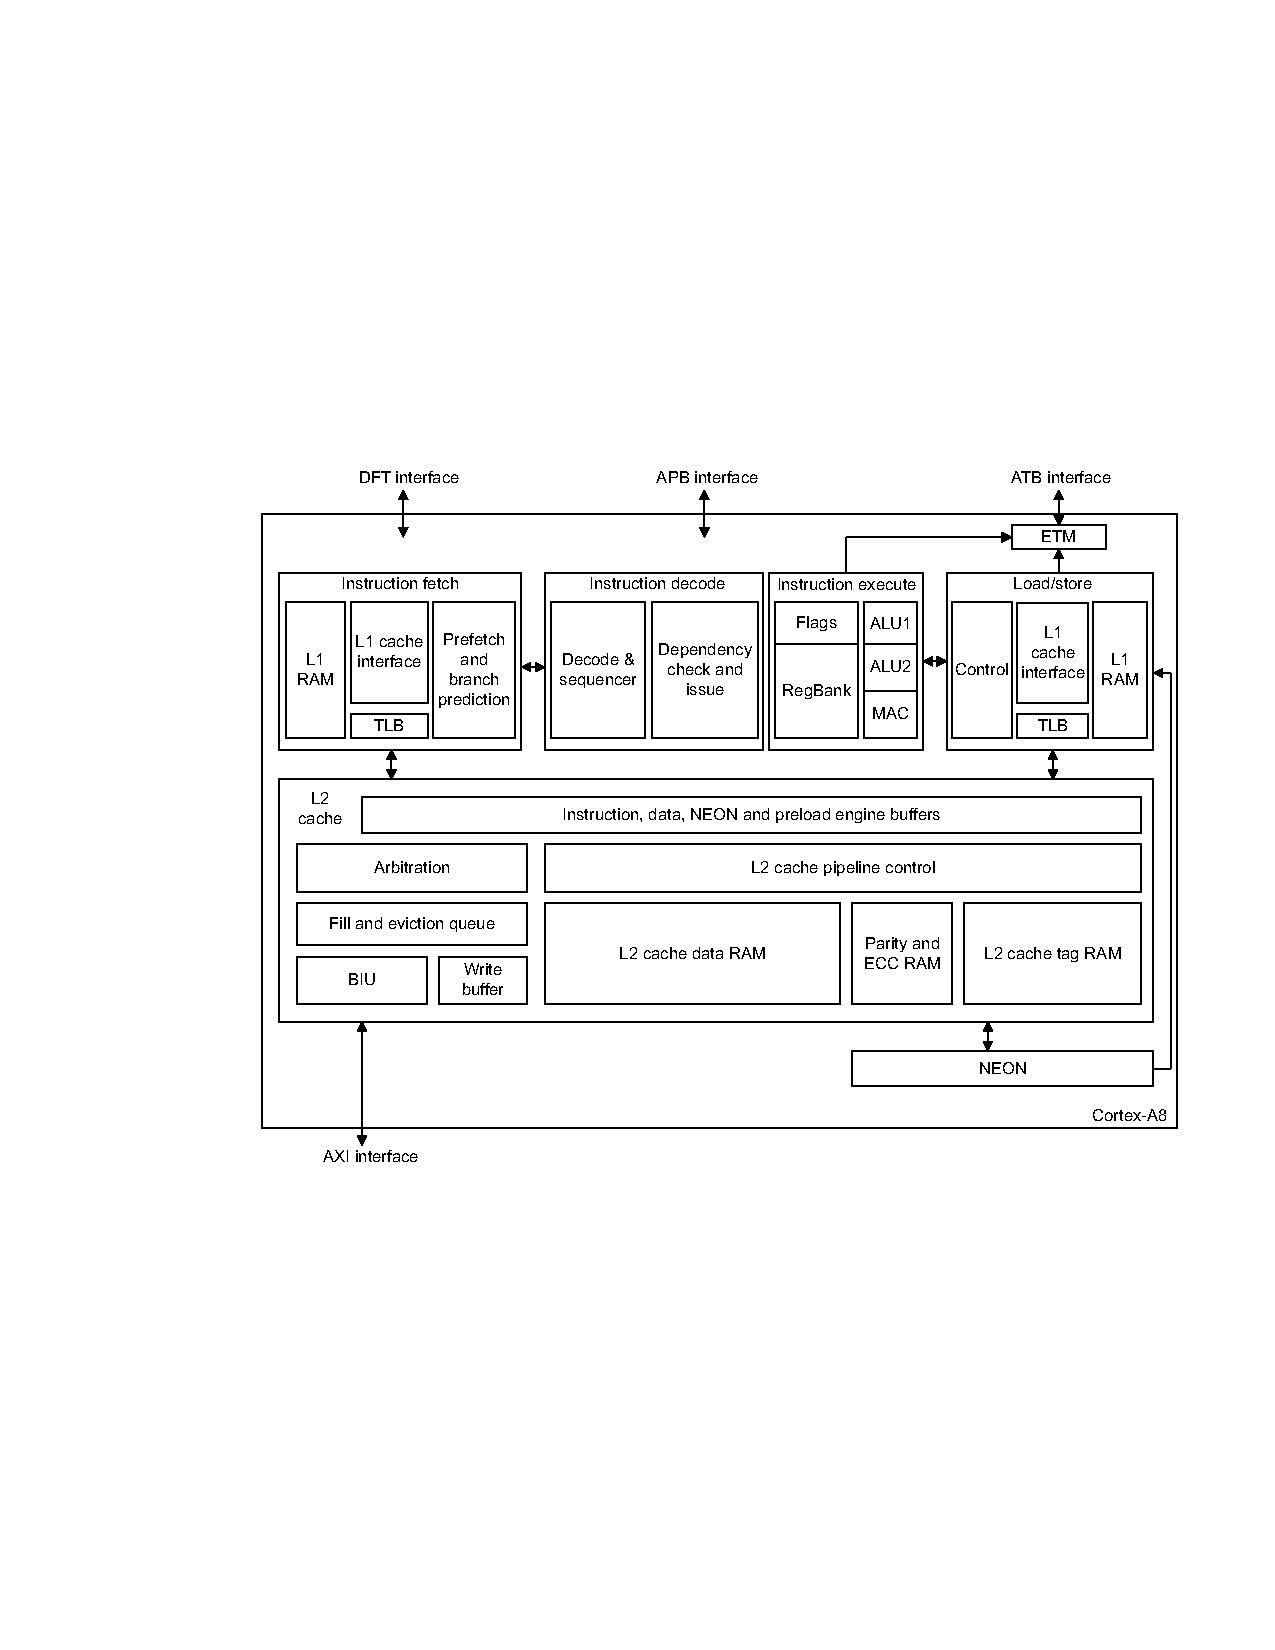
\includegraphics[width=1.0\textwidth]{./fig/CortexA8.pdf}
	\caption{Overview of the Cortex-A8 architecture from \cite[p. 1-4]{A8Ref}.}
	\label{fig:cortexa8}
\end{figure}

\chapter{Main Features}

ARM is a \emph{reduced instruction set computer} (RISC) architecture. It is a load/store architecture, meaning that its operations are performed on register contents, which are loaded from memory, and then stored back to memory; it does not perform operations directly on memory contents. It performs integer operations in a 13-stage pipeline, and floating point operations in a 10-stage NEON pipeline. The full pipeline is illustrated in Figure~\ref{fig:pipeline}.

The Cortex-A8 is a in-order, dual-issue, superscalar microprocessor core that supports the following instruction sets:
\begin{description}
	\item[ARM] is a 32-bit instruction set which includes some interesting features such as conditional execution of almost all instructions, execution of shift/rotate operations with ALU operations in the same instruction, and 2-word (64-bit) SIMD operations.
	
	\item[Thumb-2] is a variable-sized instruction set. Thumb is a 16-bit instruction subset of the ARM instruction set, created with the goal to increase code density. However, it reduced the number of available instructions so much that performance decreased, so Thumb-2 was created as a variable 16/32-bit instruction set aiming to provide ``Thumb code density at ARM performance'' \cite[p. 5]{Gris}.
	
	\item[VFPv3] (\emph{Vector Floating Point v3}) is a floating point instruction set, which is executed in the NEON unit. It supports single-word and double-word operations in its 16 double-word registers.
	
	\item[Advanced SIMD] is a SIMD instruction set that works together with VFPv3 in the NEON unit. It shares the VFPv3 registers, but can also address them as quad-word (128-bit) registers. Advanced SIMD operations can execute double-word or quad-word operands in parallel.
\end{description}

\begin{figure}[htbp]
	\centering
	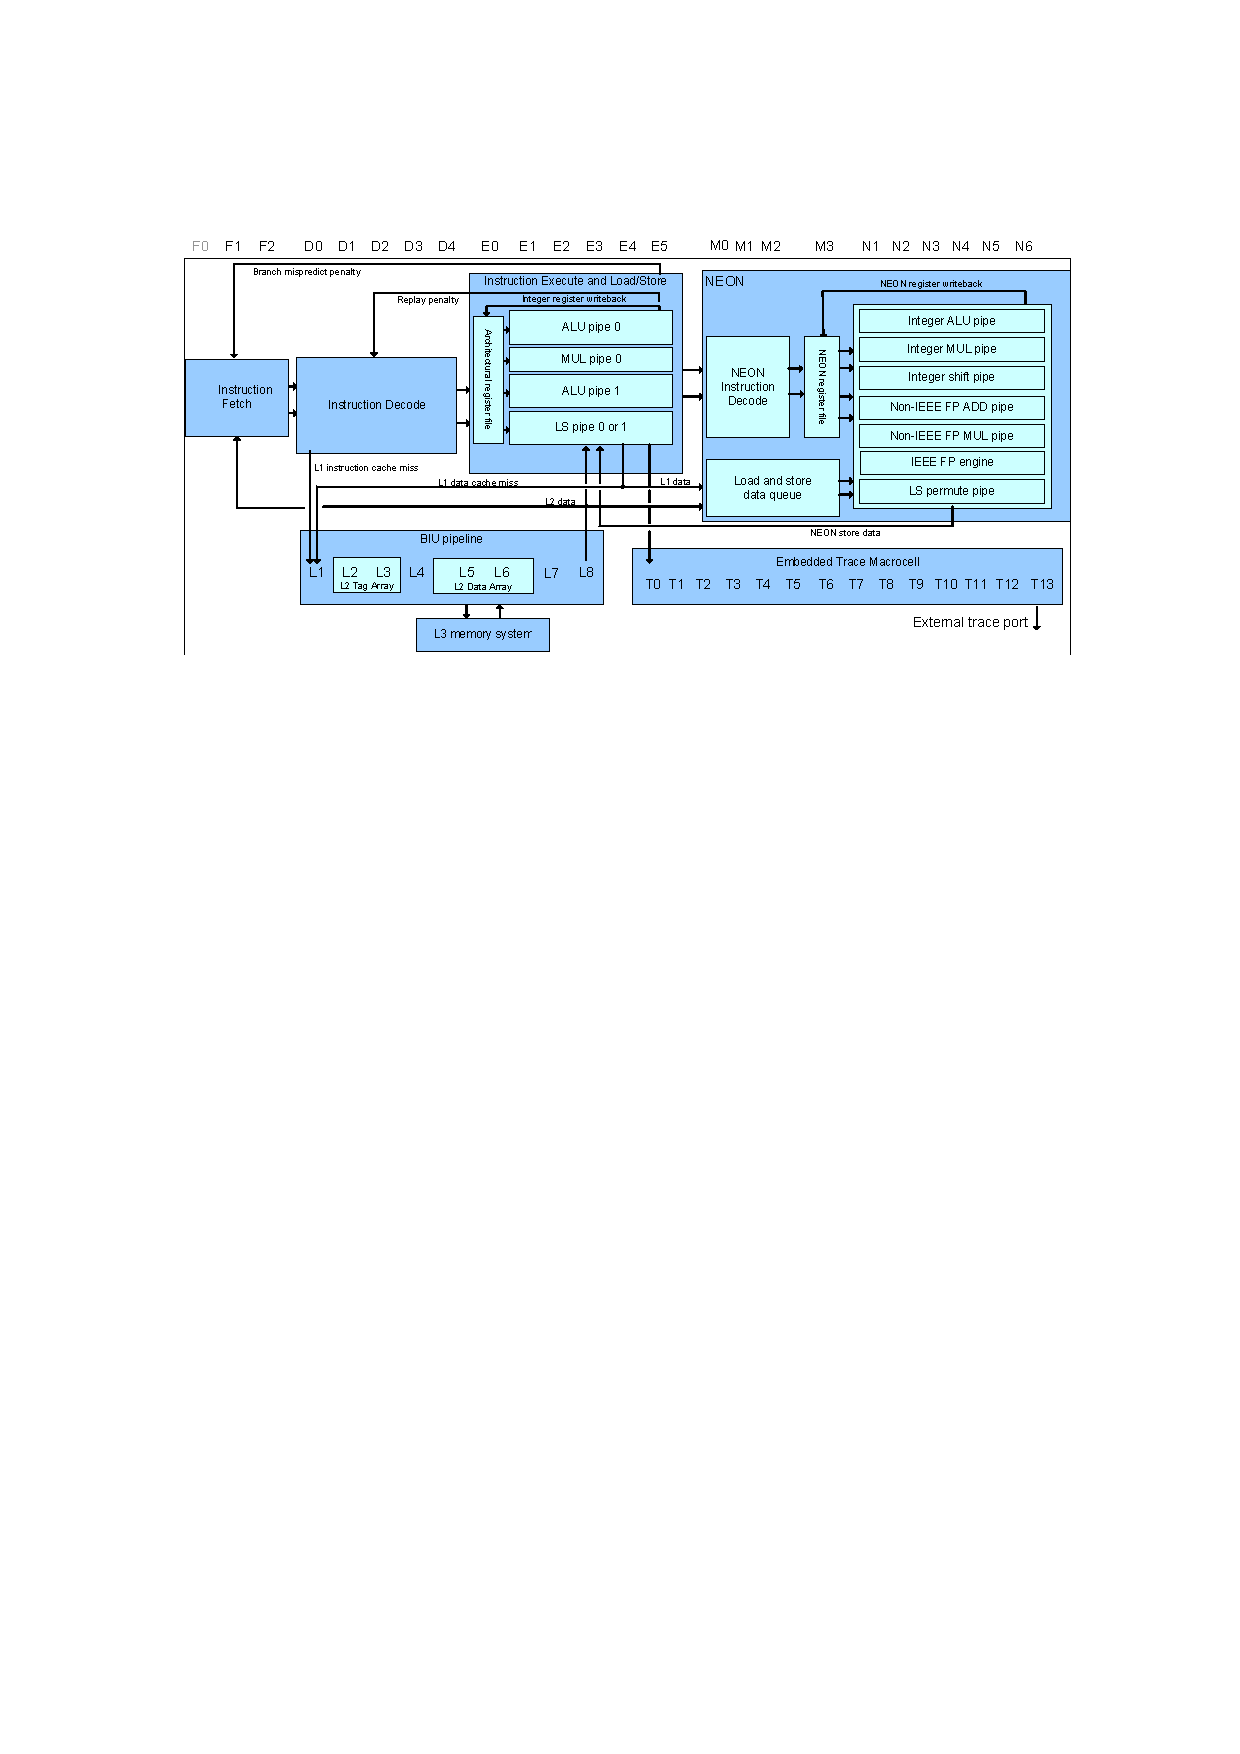
\includegraphics[width=1.0\textwidth]{./fig/Pipeline.pdf}
	\caption{Cortex-A8 full pipeline from \cite[p. 3]{Williamson}.}
	\label{fig:pipeline}
\end{figure}

\chapter{Registers}

ARM Cortex-A8 contains 16 user registers are 32 bits long. However, load and store operations are not limited to word-sized data, and these operations can be performed with bytes, half-words, words and double-words. There are also load and store operations that support two or more words of data, so it is possible to fill all registers with a single load.

The processor has 40 registers \cite[p. 2-18]{A8Ref}. This includes 33 general-purpose registers and 7 \emph{saved program status registers} (SPSRs). The format of a SPSR on a Cortex-A8 processor is illustrated in Figure~\ref{fig:cpsr}. In user-mode 16 data registers and 2 status registers are accessible, and these are described in Table~\ref{tab:registers}. Though 16 registers are available, many of these are reserved. r13, r14 and r15 are used for the stack pointer, link register and program counter, respectively. On iOS r7 is also reserved for use as the frame pointer.

\begin{figure}[htb]
	\centering
	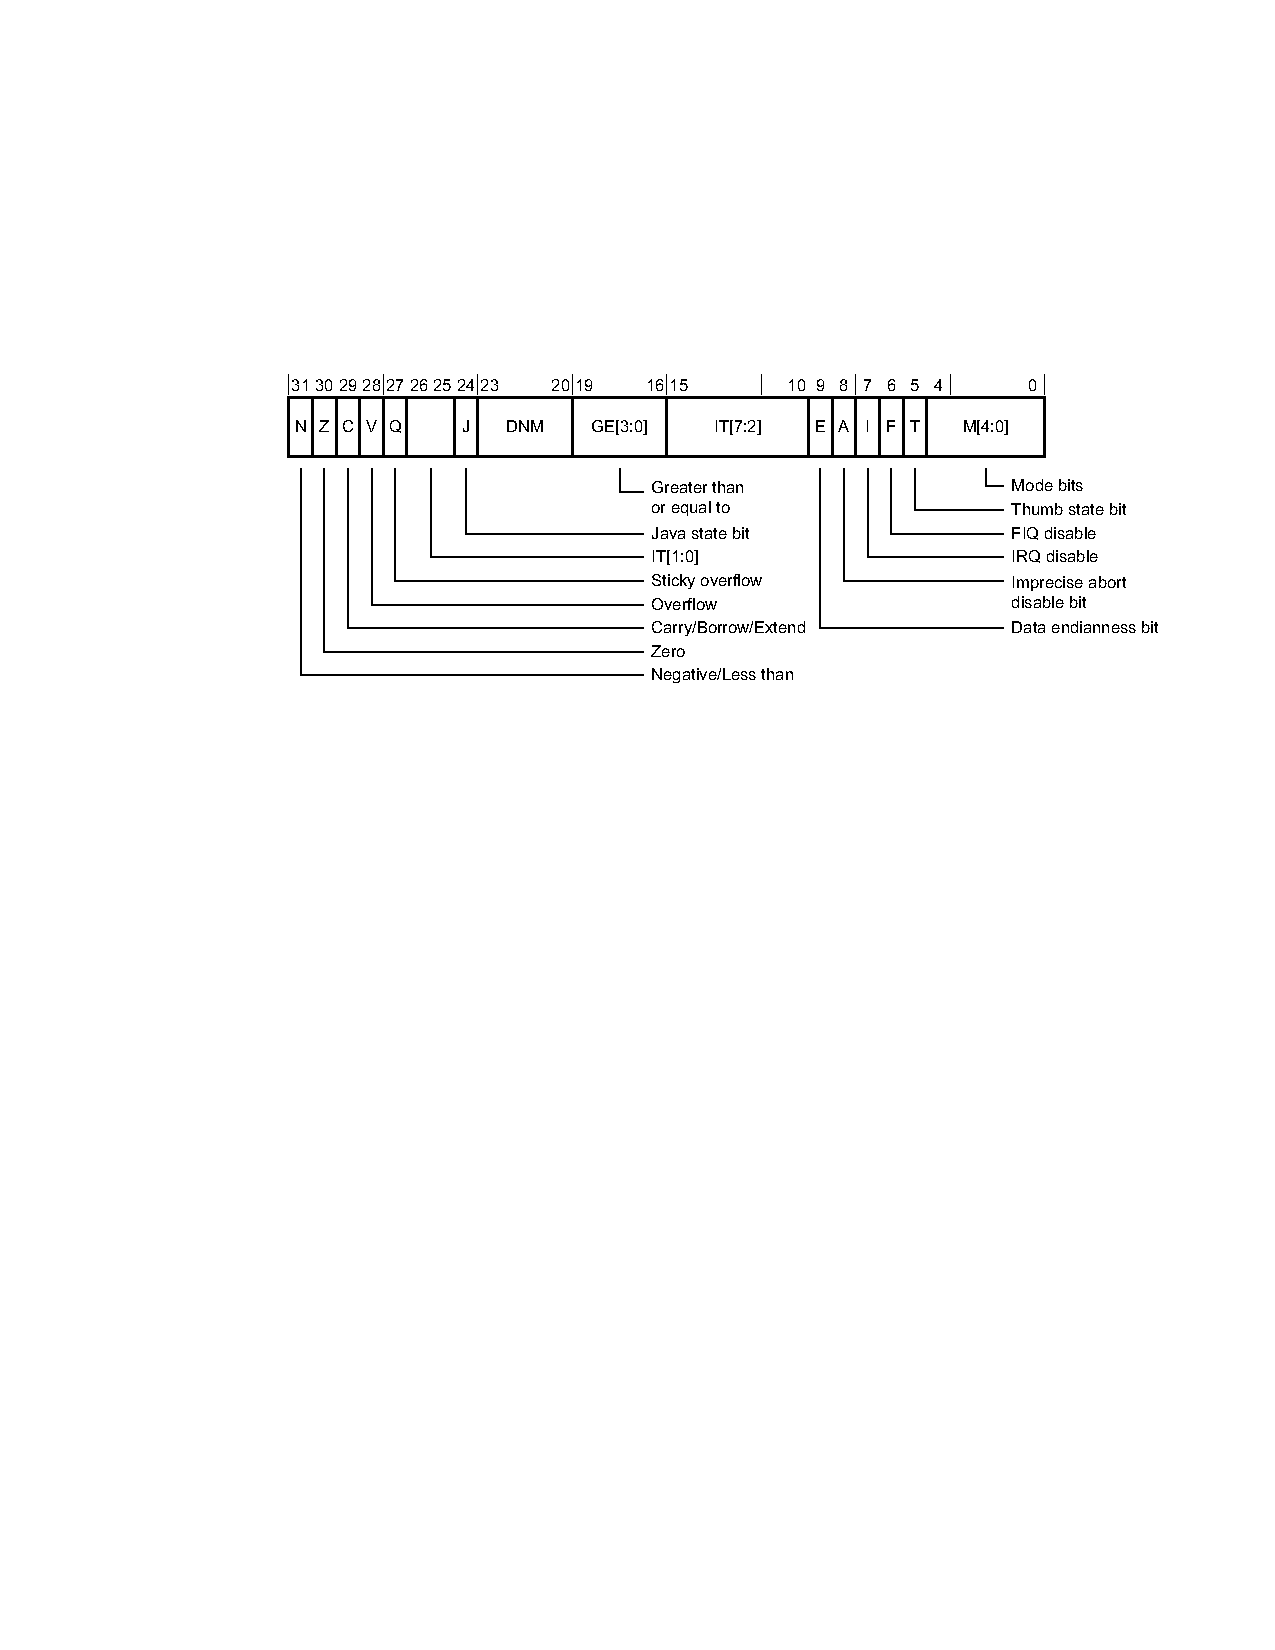
\includegraphics[width=1.0\textwidth]{./fig/CPSR.pdf}
	\caption{Program status register from \cite[p. 2-21]{A8Ref}.}
	\label{fig:cpsr}
\end{figure}

The NEON unit also has its own registers for use in VFP and NEON operations. There are 8 128-bit (quad-word) registers available. These can also be addressed as 16 double-word registers or 32 single-word registers. This is illustrated in Table~\ref{tab:registers}.

\begin{table}[p]
	\centering
	\singlespacing
		\begin{tabular}{lllllll}
		\toprule
		Type						&	\multicolumn{3}{l}{Name}	&	Preserved	&	Notes						\\
		\midrule
	 	General-purpose register	&	\multicolumn{3}{l}{R0}		&	No			&	Argument/result/scratch 1   \\
							 		&	\multicolumn{3}{l}{R1}		&	No			&	Argument/result/scratch 2   \\
							 		&	\multicolumn{3}{l}{R2}		&	No			&	Argument/scratch 3			\\
							 		&	\multicolumn{3}{l}{R3}		&	No			&	Argument/scratch 4			\\
							 		&	\multicolumn{3}{l}{R4}		&	Yes			&	Variable register 1			\\
							 		&	\multicolumn{3}{l}{R5}		&	Yes			&	Variable register 2			\\
							 		&	\multicolumn{3}{l}{R6}		&	Yes			&	Variable register 3			\\
							 		&	\multicolumn{3}{l}{R7}		&	Yes			&	Variable register 4 / Frame pointer on iOS	\\
							 		&	\multicolumn{3}{l}{R8}		&	Yes			&	Variable register 5			\\
							 		&	\multicolumn{3}{l}{R9}		&	Special		&	Platform register			\\
							 		&	\multicolumn{3}{l}{R10}		&	Yes			&	Variable register 7			\\
							 		&	\multicolumn{3}{l}{R11}		&	Yes			&	Variable register 8			\\
							 		&	\multicolumn{3}{l}{R12}		&	No			&	The Intra-Procedure-call scratch register (IP)	\\
							 		&	\multicolumn{3}{l}{R13}		&	Special		&	Stack pointer (SP)	 		\\
							 		&	\multicolumn{3}{l}{R14}		&	Special		&	Link register (LR)	 		\\
							 		&	\multicolumn{3}{l}{R15}		&	Special		&	Program counter (PC) 		\\
		Program status register		&	\multicolumn{3}{l}{CPSR}	&	Special		&						 		\\
		NEON register				&	Q0	&	D0	&	S0			&	No			&	  		\\
									&		&		&	S1			&	No			&	  		\\
									&		&	D1	&	S2			&	No			&	  		\\
									&		&		&	S3			&	No			&	  		\\
									&	Q1	&	D2	&	S4			&	No			&	  		\\
									&		&		&	S5			&	No			&	  		\\
									&		&	D3	&	S6			&	No			&	  		\\
									&		&		&	S7			&	No			&	  		\\
									&	Q2	&	D4	&	S8			&	No			&	  		\\
									&		&		&	S9			&	No			&	  		\\
									&		&	D5	&	S10			&	No			&	  		\\
									&		&		&	S11			&	No			&	  		\\
									&	Q3	&	D6	&	S12			&	No			&	  		\\
									&		&		&	S13			&	No			&	  		\\
									&		&	D7	&	S14			&	No			&	  		\\
									&		&		&	S15			&	No			&	  		\\
									&	Q4	&	D8	&	S16			&	Yes			&	  		\\
									&		&		&	S17			&	Yes			&	  		\\
									&		&	D9	&	S18			&	Yes			&	  		\\
									&		&		&	S19			&	Yes			&	  		\\
									&	Q5	&	D10	&	S20			&	Yes			&	  		\\
									&		&		&	S21			&	Yes			&	  		\\
									&		&	D11	&	S22			&	Yes			&	  		\\
									&		&		&	S23			&	Yes			&	  		\\
									&	Q6	&	D12	&	S24			&	Yes			&	  		\\
									&		&		&	S25			&	Yes			&	  		\\
									&		&	D13	&	S26			&	Yes			&	  		\\
									&		&		&	S27			&	Yes			&	  		\\
									&	Q7	&	D14	&	S28			&	Yes			&	  		\\
									&		&		&	S29			&	Yes			&	  		\\
									&		&	D15	&	S30			&	Yes			&	  		\\
									&		&		&	S31			&	Yes			&	  		\\
		VFP status register			&	\multicolumn{3}{l}{FPSCR}	&	Special		&						 		\\
		\bottomrule
	\end{tabular}
	\caption{User-mode registers. Compiled from \cite[p. 15]{AAPCS} and \cite[p. 14--15]{iOSABI}.}
	\label{tab:registers}
\end{table}

\chapter{Data Types}

There are four data types available for arithmetic operations in ARM mode \cite[p. 2-14]{A8Ref}. These are listed in Table~\ref{tab:datatypes}.

\begin{table}[htb]
	\centering
	\begin{tabular}{lr}
		\toprule
		Type			&		Size		\\
		\midrule
		doubleword		&		64-bit		\\
		word			& 		32-bit		\\
		halfword 		& 		16-bit		\\
		byte 			& 		8-bit		\\
		\bottomrule
	\end{tabular}
	\caption{ARM data types.}
	\label{tab:datatypes}
\end{table}

Data can be signed (two's complement) or unsigned, and can be little- or big-endian ordered \cite[p. 4-2]{A8Ref}. The data order is indicated in the E-bit in the Application Program Status Register (APSR). This can been seen in Figure~\ref{fig:cpsr} as \emph{E: Data endianness bit}.

Data access does not have to be aligned but for best performance data access should be word-aligned.

\chapter{Instruction Format}

ARM instructions are 32-bit, little-endian format. There are many different types of instruction, and each of these has a different format. These formats are illustrated in Figure~\ref{fig:instructionformat}.

Thumb instructions are 16 bits long, and Thumb-2 instructions are variable length of 16- and 32-bit.

\begin{figure}[htbp]
	\centering
	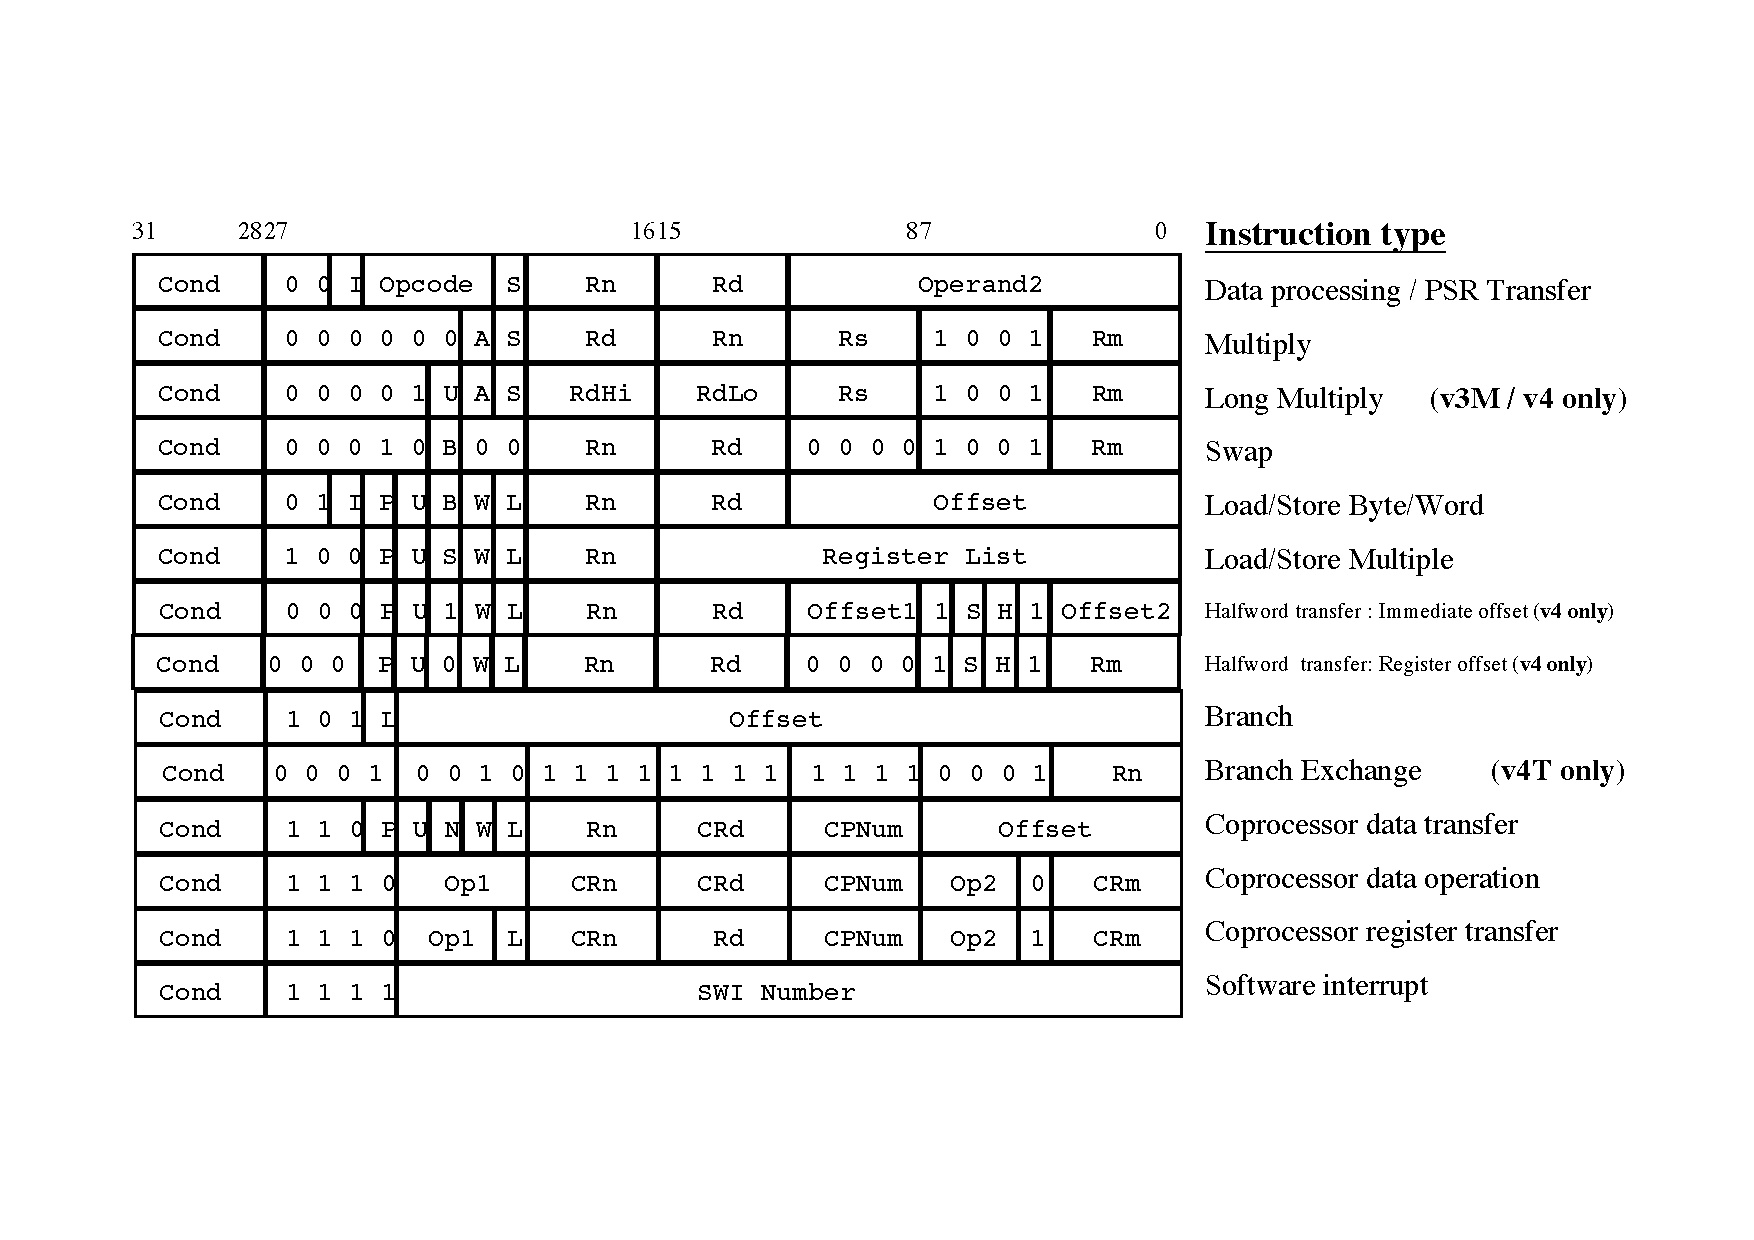
\includegraphics[width=1.0\textwidth]{./fig/InstructionFormat.pdf}
	\caption{ARM instruction set format from \cite[p. 13]{ARMInst}.}
	\label{fig:instructionformat}
\end{figure}

\section{Unified Assembler Language}
ARM provides the \emph{Unified Assembler Language} (UAL) as a canonical language for all ARM and Thumb commands. Assembly written in UAL can be assembled to ARM alone, or to ARM with Thumb, depending on the target processor.

\section{Condition Codes}
An interesting feature of ARM instructions is their conditional bits, which can be seen in Figure~\ref{fig:instructionformat} as bits 31--28. In UAL, ARM instructions that end in \texttt{S} (for example \texttt{ADDS} vs. \texttt{ADD}, and \texttt{SUBS} vs. \texttt{SUB}) set the condition flags in the APSR (bits 31--28). The value of these four bits together with the state of the condition flags in the APSR determine whether or not the instruction is executed. The different condition codes are listed in Figure~\ref{fig:conditioncodes}. Even if not executed the instruction still uses one cycle.

\begin{figure}[htb]
	\centering
	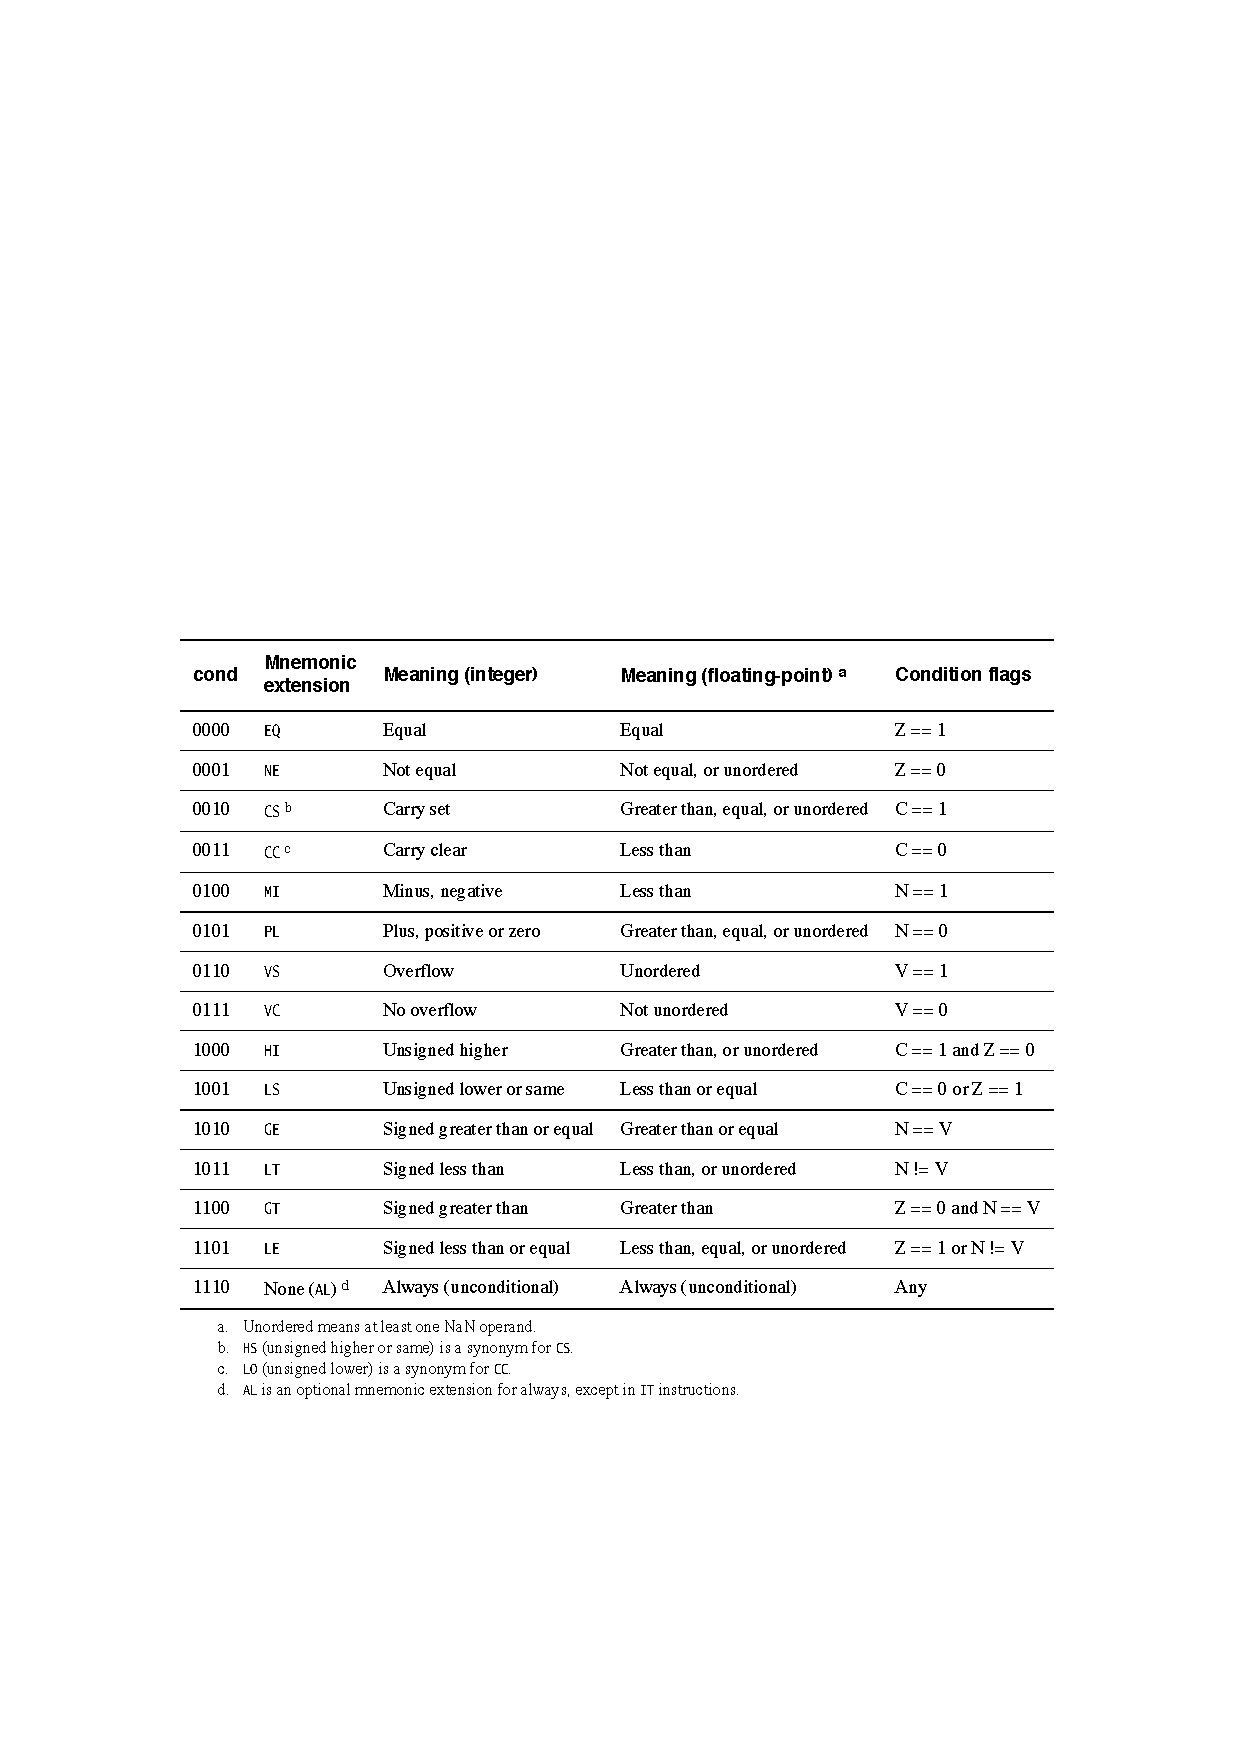
\includegraphics[width=1.0\textwidth]{./fig/ConditionCodes.pdf}
	\caption{Condition codes from \cite[p. A8-8]{ARMRef}.}
	\label{fig:conditioncodes}
\end{figure}

\section{Barrel Shifter}
ARM provides shift and rotate operations, but these can be performed as part of other data processing instructions.

There are four basic instructions, shown in Table~\ref{tab:shifts}. The parameter $n$ can either be an immediate constant (a constant prefixed by \texttt{\#}), or can be a register. In the case of a register, the bottom byte is used to determine the parameter and an extra cycle is required \cite[p. 31]{ARMInst}.

\begin{table}[htb]
	\centering
	\begin{tabular}{lll}
		\toprule
		Operation		&	Description				&	$n$ Range		\\
		\midrule
		\texttt{LSL}	$n$			&	Logical shift left		&	$1 <= n <= 31$	\\
		\texttt{LSR}	$n$			&	Logical shift right		&	$1 <= n <= 32$	\\
		\texttt{ASR}	$n$			&	Arithmetic shift right	&	$1 <= n <= 32$	\\
		\texttt{ROR}	$n$			&	Rotate right			&	$1 <= n <= 31$	\\
		\bottomrule
	\end{tabular}
	\caption{Barrel shifter operations. \cite[p. A8-10]{ARMRef}}
	\label{tab:shifts}
\end{table}

The barrel shifter increases code density. To demonstrate this, let us see an example of a simple arithmetic operation:

$r_0 = r_1 + 8\cdot{}r_2$

Without using the barrel shifter, this could be implemented with two instructions (and two cycles) as so:

\begin{singlespacing}
\begin{lstlisting}[language={[ARM]Assembler}]
mul r0, r2, #8           // r0 = r2 * 8
add r0, r1               // r0 = r0 + r1
\end{lstlisting}
\end{singlespacing}

However, using the barrel shifter we can reduce this to one instruction, which is executed in one cycle.

\begin{lstlisting}[language={[ARM]Assembler}]
add r0, r1, r2, LSL #3   // r0 = r1 + (r2 << 3)
\end{lstlisting}

A4
A5.1

\chapter{Unusual Instructions}
Perhaps in A4.4.6, A4.4.7, A4.8
bit fields?

\chapter{Memory Management}

\section{Programmer's Model}

As ARM is a \emph{Load/Store Architecture}, it does not perform operations directly on memory. Before any operation is performed, the memory must first be \emph{loaded} into registers, and when the operation is completed, the result must be \emph{stored} back into memory. 

\begin{table}[htb]
	\begin{tabular}{lll}
		\toprule
		Data length	&	Load instruction(s)								&	Store operation(s)								\\
		\midrule
		Multiple	&	\texttt{LDM} / \texttt{LDMIA} / \texttt{LDMFD}	&	\texttt{STM} / \texttt{STMIA} / \texttt{STMEA}	\\
		Dual		&	\texttt{LDRD}									&	\texttt{STRD}									\\
		Word		&	\texttt{LDR}									&	\texttt{STR}									\\
		Half-word   &	\texttt{LDRH} / \texttt{LDHRS}					&	n/a												\\
		Byte        &	\texttt{LDRB} / \texttt{LDRSB}					&	n/a												\\
		\bottomrule		
	\end{tabular}
	\caption{Load and store instructions for various data types.}
	\label{tab:loadstore}
\end{table}

Note that load instructions that read data types shorter than word length have signed and unsigned variants. This is necessary because the data will be extended to a word-length type when loaded. For the same reason, note that these data types have no store operations. Once loaded they are word-length types which can be stored with \texttt{STR}, \texttt{STRD}, \texttt{STM}, etc.

\subsection{Auto-incrementing}
The commands listed above can be used with auto-incrementing functionality. This can be seen by use of the \texttt{!} symbol in the code in Figure~\ref{fig:autoincrement} which demonstrates a simple \texttt{memcpy()} implementation.

\begin{figure}[htb]
	\centering
	\begin{lstlisting}[language={[ARM]Assembler}]
// r12 points to the start of the source data
// r14 points to the end of the source data
// r13 points to the start of the destination data loop
ldmia r12!, {r0-r11}    // load 48 bytes, add 48 to r12
stmia r13!, {r0-r11}    // and store them, add 48 to r13
cmp r12, r14            // check for the end
bne loop                // and loop until done
	\end{lstlisting}
	\caption{Example of auto-incrementing addressing adapted from \cite[p. 61]{ARMInst}.}
	\label{fig:autoincrement}
\end{figure}

\section{Implemention}

The Cortex-A8 uses a multilevel memory hierarchy, with L1 and L2 cache available for high-speed access and external L3 memory (DRAM, SRAM, Flash, ROM, etc) available over the AXI interface (seen in Figure~\ref{fig:cortexa8}). The arrangement of these various levels of cache is shown in Figure~\ref{fig:memoryhierarchy}.

\begin{figure}[hb]
	\centering
	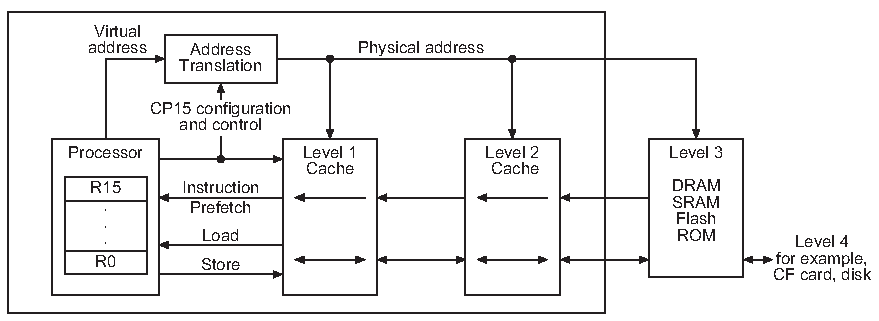
\includegraphics[width=1.0\textwidth]{./fig/MemoryHierarchy.pdf}
	\caption{Memory hierarchy from \cite[p. A3-52]{ARMRef}}
	\label{fig:memoryhierarchy}
\end{figure}

\subsection{Virtual Memory System Architecture (VMSA)}
The Cortex-A8, as with all ARMv7-A architecture processors, uses the \emph{Virtual Memory System Architecture} (VMSA) to provide virtual memory addressing. A VMSA's \emph{Memory Management Unit} (MMU) controls allocation of dynamic memory and the mapping of virtual addresses to physical addresses \cite[p. B3-2]{ARMRef}.


\subsection{L1 Cache}

The Cortex-A8's L1 memory system is a Harvard architecture: it contains separate one instruction and data caches \cite[p. 7-2]{A8Ref}. It has parity checking to detect errors, and has both blocking and nonblocking cache behaviours for integer and Advanced SIMD code, respectively.

The instruction cache is indexed virtually with the IVIPT extension (\emph{Instruction cache Virtually Indexed Physically Tagged extension}), which is designed to simplify instruction cache maintenance by only requiring a single condition: updating data at an instruction address \cite[p. 7-4]{A8Ref}. Data cache is indexed physically (\emph{Physically Indexed, Physically Tagged}, PIPT), but this is much slower than the VIPT instruction cache because the physical address must be looked up, and in doing so if a \emph{translation lookaside buffer} (TLB) miss is encountered external memory must be accessed \cite[p. 7-8]{A8Ref}.

A3
B2

6-2
\chapter{ARM Assembly Example}
An example of ARM assembly programming can be seen in Appendix~\ref{appendix:a} (p. \pageref{appendix:a}).

This code calculates the inner product of two $n$-length vectors. Functions are provided for 32-bit signed integer vectors and floating point vectors.

\section{Interface}

In C, these two functions are declared respectively as follows.

\begin{singlespacing}
\begin{lstlisting}[language={AssemblerC}]
int32_t dot_product_int32_asm(int32_t *,int32_t *, int32_t);
float dot_product_float_asm(float *,float *, int32_t);
\end{lstlisting}
\end{singlespacing}

For the purposes of reference and benchmarking, the following C implementations were created.

\begin{singlespacing}
\begin{lstlisting}[language={AssemblerC}]
int32_t dot_product_int32(int32_t *x,int32_t *y, int32_t n) {
    int32_t sum = 0;
    while (--n >= 0) sum += x[n] * y[n];
    return sum;
}

float dot_product_float(float *x,float *y, int32_t n) {
    float sum = 0.0f;
    while (--n >= 0) sum += x[n] * y[n];
    return sum;
}
\end{lstlisting}
\end{singlespacing}

Additionally, the floating point implementation has a secondary reference implementation that takes advantage of Advanced SIMD using Apple's Accelerate framework \cite{Accelerate}.

\begin{singlespacing}
\begin{lstlisting}[language={AssemblerC}]
float dot_product_float_accelerate(float *x,float *y, int32_t n) {
    float result;
    vDSP_dotpr(x, 1, y, 1, &result, n);
    return result;
}
\end{lstlisting}
\end{singlespacing}

\section{Implementation}
iOS ABI Function Call Guide \cite{iOSABI}

\section{Benchmarking}

To test the performance of the ARM assembly implementation random vectors were generated of varying lengths and their dot products were calculated in all implementations (C Signed 32-bit Integer, ARM Signed 32-bit Integer, C Float, ARM Float, vDSP Float). The vector lengths used were 10, 100, 500, 1,000, 2,000, 4,000, 8,000, 16,000, 32,000, 64,000, 128,000, 256,000 and 512,000.

The results can be seen in detail in Table~\ref{tab:results} and are charted in Figure~\ref{fig:results}. There are a few interesting things to note in these results:
\begin{enumeration}
	\item The C implementations are a whole magnitude of order slower than the other implementations.
	\item The asm implementations are accelerated by NEON, but the vDSP implementation is still faster. The asm implementations' use of NEON is restricted to 8 elements at a time, but by using more NEON registers it is possible to decrease the amount of branching, and therefore keep the pipeline full for longer.
\end{enumeration}

\begin{figure}[htb]
	\centering
	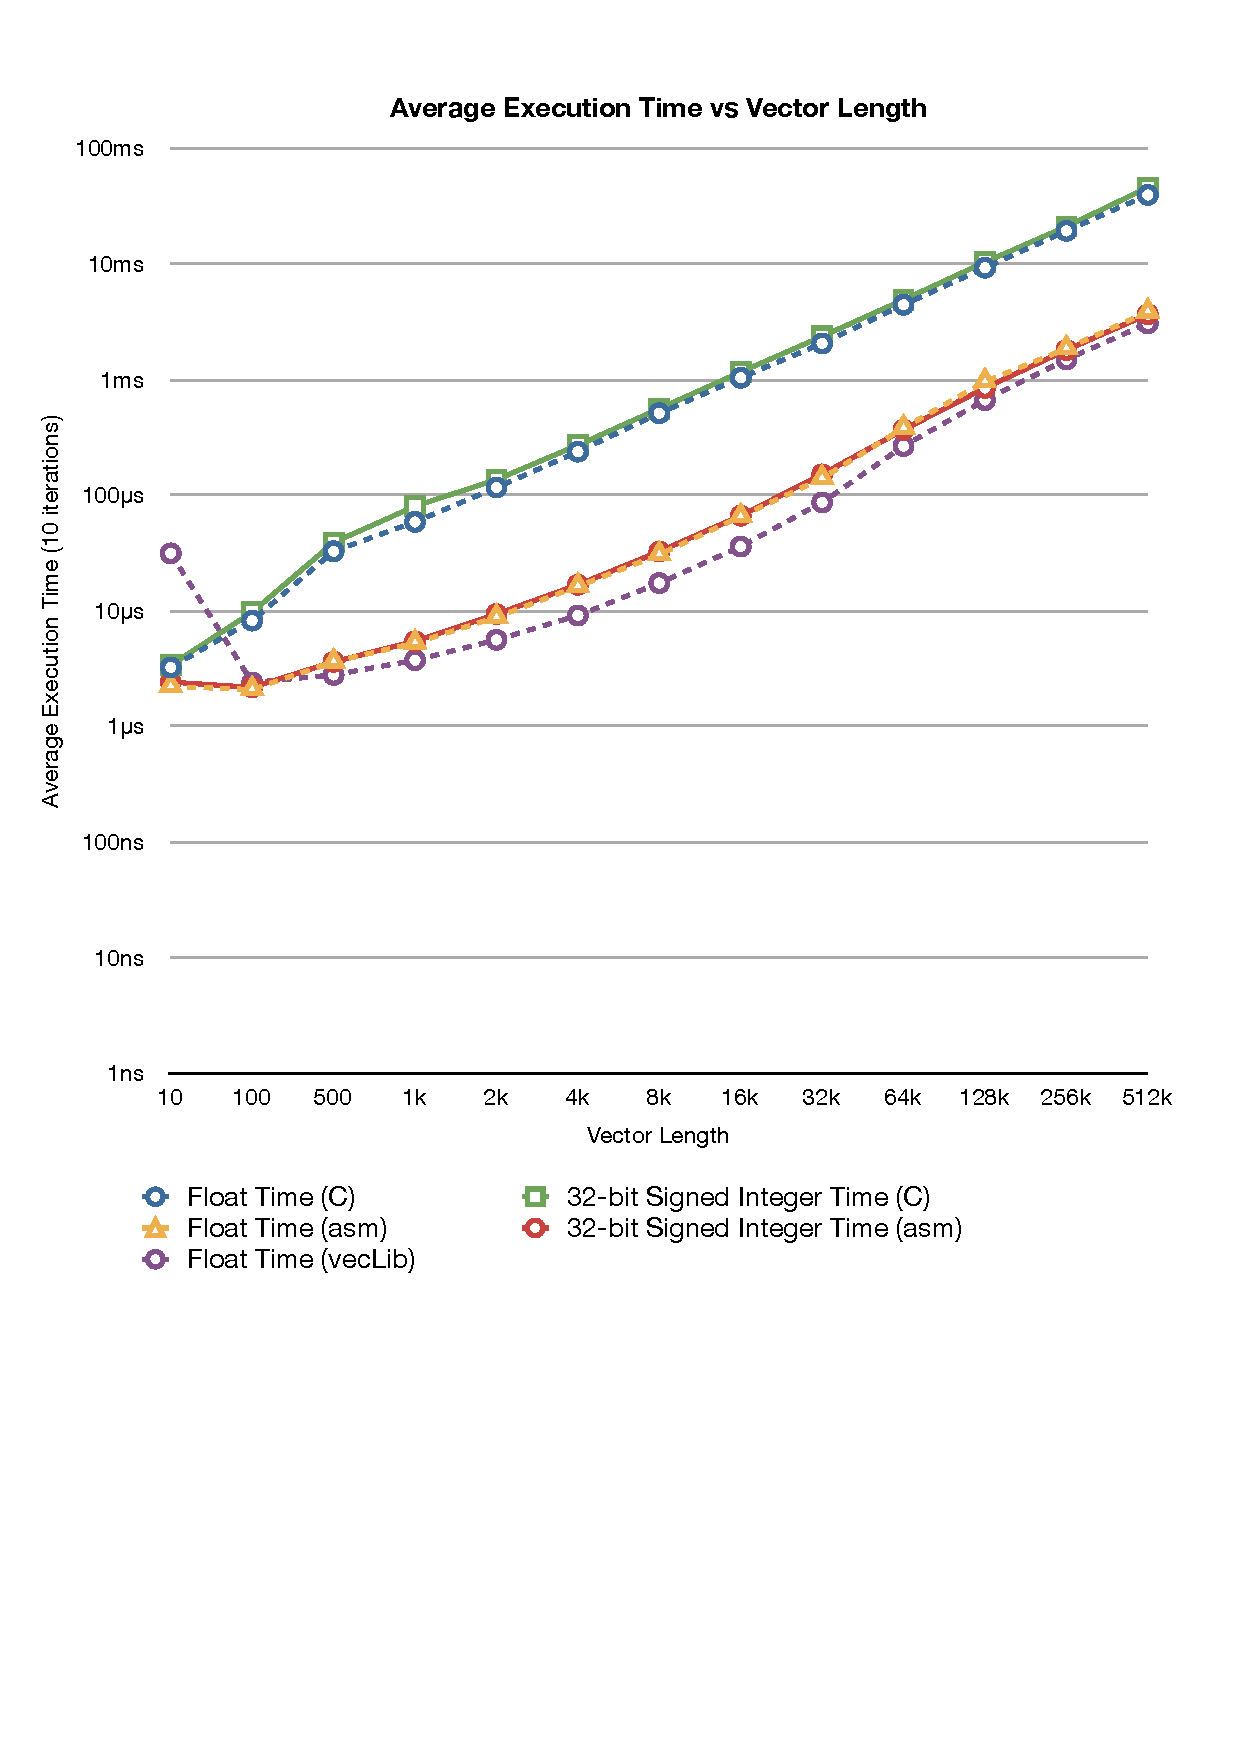
\includegraphics[width=1.0\textwidth]{./fig/ResultsChart.pdf}
	\caption{\ldots}
	\label{fig:results}
\end{figure}

\begin{table}[htb]
	\centering
	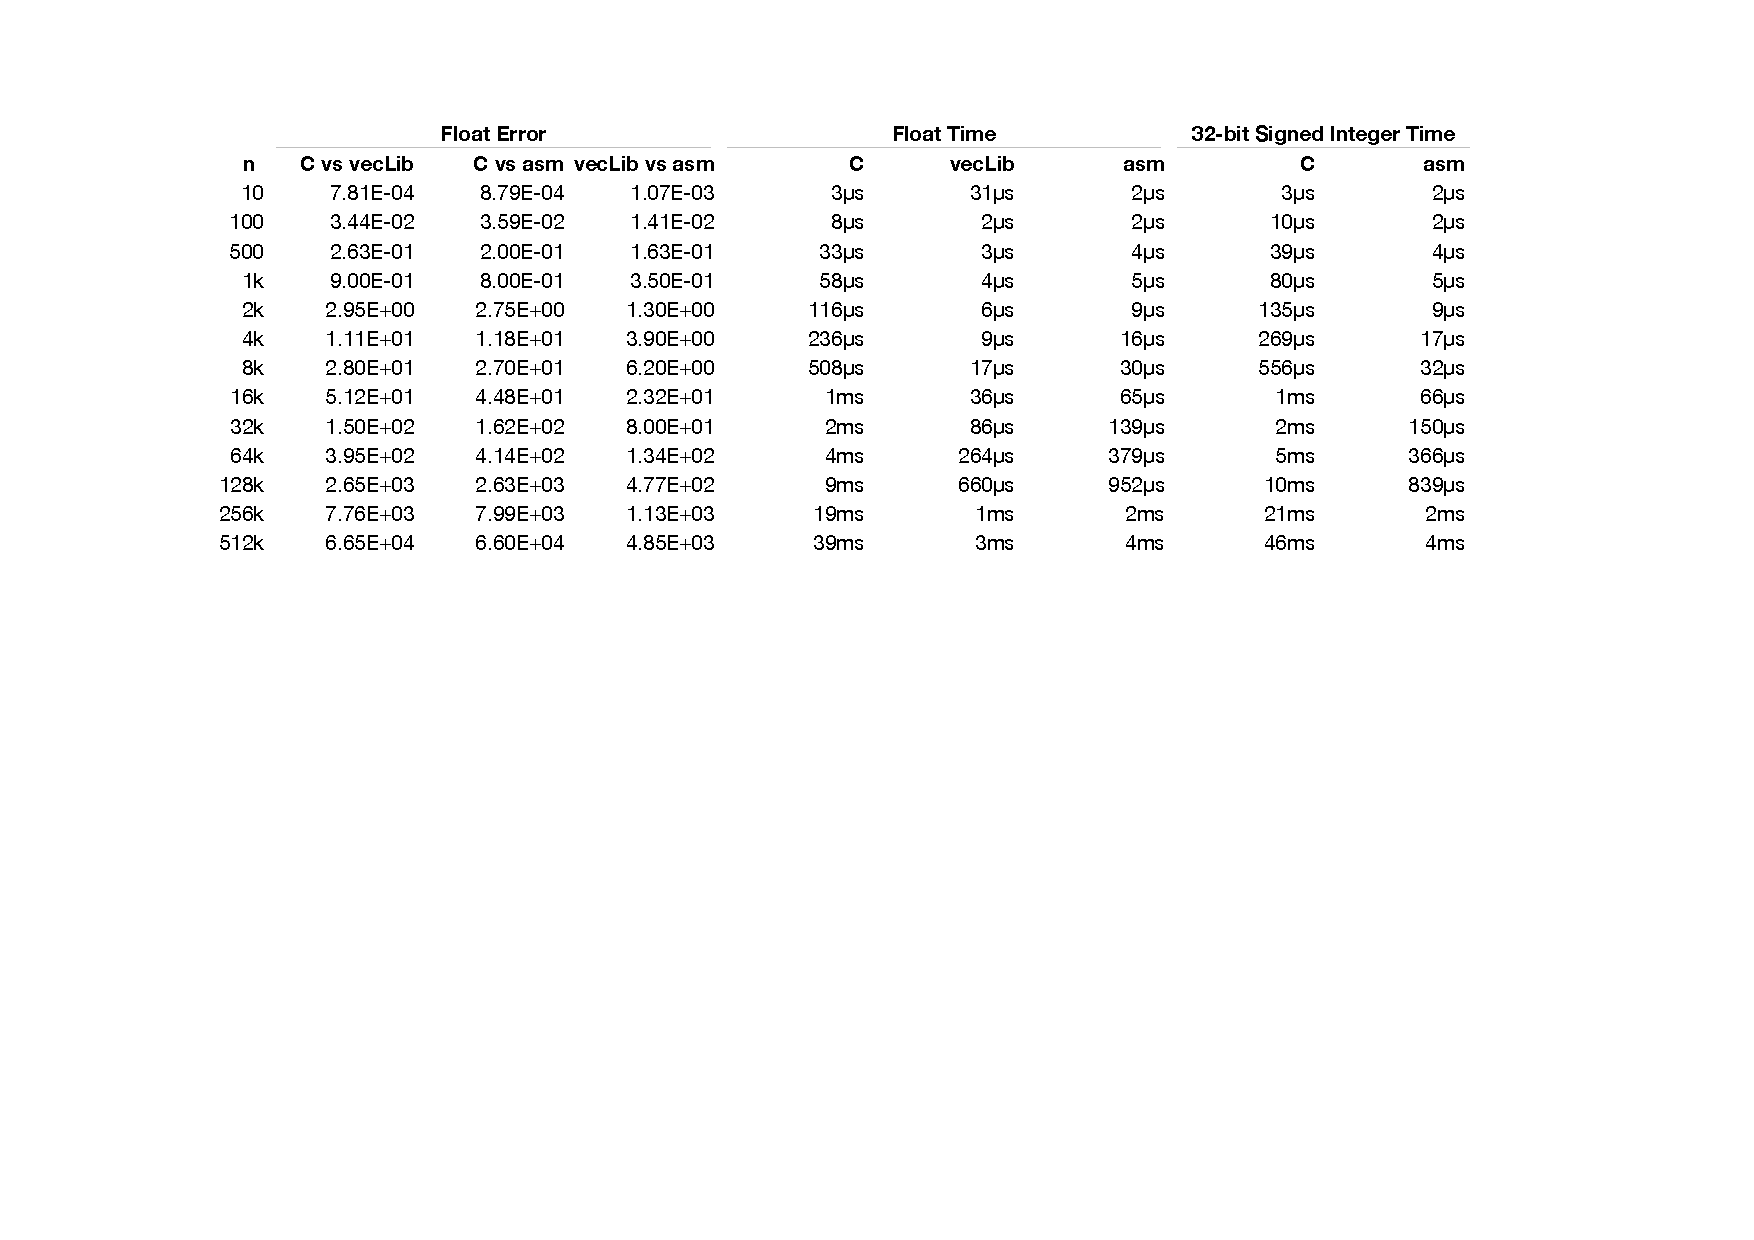
\includegraphics[width=1.0\textwidth]{./fig/ResultsTable.pdf}
	\caption{\ldots}
	\label{tab:results}
\end{table}

\bibliographystyle{plain}
\bibliography{ARM_Report}

\clearpage

\appendix
\chapter{ARM Assembly Programming Example -- Inner Product of Two Vectors}\label{appendix:a}

\begin{singlespacing}
\lstinputlisting[language={[ARM]Assembler}]{../ARM/dot_product.s}	
\end{singlespacing}  

\end{document}
